\chapter{System Kelvin}
\label{ch:kelvin}

Tato kapitola se věnuje školnímu systému Kelvin (\href{https://kelvin.cs.vsb.cz/}{https://kelvin.cs.vsb.cz/}), který slouží jako základní platforma pro odevzdávání a hodnocení programátorských úloh.
Cílem kapitoly je přiblížit účel systému, jeho architekturu, způsob nasazení a především vývojová omezení, která významně ovlivnila návrh a implementaci řešení popsaného v této diplomové práci.

% =============================================================
\section{Účel systému}
\label{sec:kelvin-purpose}

Hlavním účelem systému Kelvin je podpora výuky, především programovacích předmětů v jazycích C, C++, Python nebo Rust, ale slouží také jako obecný systém pro odevzdávání úloh v dalších předmětech jakou jsou základy počítačové grafiky (ZPG), modelování v grafických aplikacích (MGA) a další.
Systém poskytuje jednotné webové rozhraní, prostřednictvím kterého mohou studenti odevzdávat svá řešení úloh.
Vyučujícím následně umožňuje tato řešení kontrolovat, poskytovat k nim zpětnou vazbu a udělovat bodové hodnocení.
Součástí systému jsou také moduly pro automatické přeložení odevzdaného kódu, jeho spuštění a ověření výstupů.

\subsection{Typický scénář použití}
\label{subsec:kelvin-workflow}

Cyklus jedné úlohy v systému Kelvin zahrnuje několik na sebe navazujících kroků, od vytvoření zadání vyučujícím až po závěrečné manuální hodnocení odevzdaného řešení:

Vyučující nejprve vytvoří úlohu, kde zadá její textový popis, definuje testovací vstupy, očekávané výstupy a nastaví termín odevzdání.
Úloha je pak zpřístupněna přihlášeným studentům okamžitě nebo v předem stanoveném čase.

Student si zadání přečte, během přiděleného času vypracuje řešení ve svém vývojovém prostředí a výsledný zdrojový kód odevzdá prostřednictvím webového rozhraní systému.
Bezprostředně po odevzdání systém spustí automatizované testy.
Systém zkompiluje zdrojový kód a spustí jej proti připraveným testovacím vstupům, následné výsledky jsou porovnány s očekávanými výstupy.
Student okamžitě vidí výsledky testů které prošly i ty, které selhaly a následně může na základě zpětné vazby řešení opravit a odevzdat znovu.

Po uzavření termínu odevzdání přistoupí vyučující k manuálnímu hodnocení.
Prohlíží zdrojový kód odevzdaného řešení přímo v prostředí systému, přidává podle svého hodnocení komentáře ke konkrétním řádkům nebo blokům kódu a na základě celkového posouzení udělí bodové hodnocení.
Student hodnocení a komentáře obdrží a může na ně reagovat, čímž může vznikat diskuse nad zdrojovým kódem a jeho kvalitou.

\endinput

\subsection{Další formy hodnocení}
\label{subsec:kelvin-other-assessments}

Systém Kelvin je rovněž využíván pro testy, kvízy a jiné formy hodnocení, které nemusí nutně zahrnovat zdrojový kód.
Například pro testování teoretických znalostí nebo algoritmického myšlení prostřednictvím krátkých formulářových nebo textových odpovědí.

\endinput

\input{chapters/2-kelvin/2-1-kelvin-purpose/2-1-3-kelvin-purpose-features}

% =============================================================
\section{Architektura systému}
\label{sec:kelvin-architecture}

Systém Kelvin je realizován jako webová aplikace se standardním třívrstvým uspořádáním: databázová vrstva, backendová aplikační logika a frontendová prezentační vrstva.
Komunikace mezi frontendem a backendem probíhá přes REST API (Representational State Transfer, Application Programming Interface)\@.

\subsection{Backend}
\label{subsec:kelvin-backend}

Backend systému je implementován v programovacím jazyce Python s využitím webového frameworku Django.
Django zajišťuje správu databázových modelů prostřednictvím ORM (Object-Relational Mapping), autentizaci a autorizaci uživatelů, správu souborů (odevzdaných zdrojových kódů a testovacích dat) a základní routování požadavků.

Použitým databázovým systémem je PostgreSQL, přičemž veškerý přístup k němu probíhá výhradně přes Django ORM\@.
Soubory zdrojových kódů jsou ukládány na souborový uložišti serveru, přičemž v databázi jsou uloženy pouze metadata (cesty, časové razítka, vazby na studenty a úlohy).

\subsubsection*{Evaluační pipeline}
\label{subsubsec:kelvin-evaluation-pipeline}

Stávající evaluační pipeline systému zajišťuje kompilaci odevzdaného zdrojového kódu a spuštění automatických testů v izolovaném prostředí.
Izolace je realizována prostřednictvím kontejnerů (Docker) a omezení přístupu k systémovým zdrojům, což chrání infrastrukturu před škodlivým nebo nekorektním kódem a současně garantuje jednotné podmínky evaluace pro všechny studenty.

Vyhodnocení je implementováno jako asynchronní úloha z pohledu aplikační architektury, nicméně z hlediska uživatelského chování se jedná o proces synchronní, protože student čeká na jeho dokončení před zobrazením výsledků testů.

Zařazení dalších výpočetně náročných operací přímo do této pipeline, například generování analýzy pomocí LLM, by vedlo k prodloužení doby čekání na výsledek.
I pokud by byly tyto operace realizovány technicky asynchronně, jejich začlenění do stejného evaluačního procesu by mělo přímý dopad na vnímanou latenci systému uživatelem.

\subsubsection*{Kontrola plagiátorství}
\label{subsubsec:kelvin-plagiarism-check}

Vedle evaluační pipeline systém Kelvin provádí rovněž kontrolu plagiátorství.
Ta je ze své podstaty vázána na celou skupinu odevzdání, nikoli na jedno konkrétní, a je proto spouštěna buď manuálně učitelem, nebo automaticky po vypršení termínu odevzdání dané úlohy.
Po spuštění systém porovná každé odevzdání s každým ostatním ve skupině za využití nástrojů DOLOS~\cite{dolos} a MOSS~\cite{moss}.
Díky tomuto uspořádání kontrola plagiátorství nijak neovlivňuje dobu čekání studentů na výsledky automatických testů.

\endinput

\subsection{API vrstva}
\label{subsec:kelvin-api}

Komunikace mezi frontendem a backendem probíhá prostřednictvím REST API implementovaného za pomocí knihovny Django Ninja.
Django Ninja je moderní framework pro budování API nad Django, inspirovaný FastAPI, který využívá Python \textit{type hints} pro automatickou validaci vstupních dat a generování OpenAPI dokumentace přístupnou například přes Swagger UI\@.

\endinput

\subsection{Frontend}
\label{subsec:kelvin-frontend}

Frontendová část systému je z technologického hlediska výrazně komplikovanější než backend, protože v době psaní práce prochází historickým vývojem, který zanechal vrstvení tří různých technologií v jednom projektu.

Nejstarší vrstvou jsou Django šablony (\textit{Django templates}) -- serverově generované HTML stránky, které byly původním způsobem tvorby uživatelského rozhraní.
Django šablony jsou stále přítomny v systému u statičtějších částí rozhraní, kde není potřeba dynamického chování na straně klienta.

Druhou vrstvou je \textit{Svelte} -- moderní JavaScript framework pro tvorbu reaktivních komponent na straně klienta.
V průběhu vývoje systému Kelvin byl Svelte adoptován jako primární framework pro dynamické části rozhraní, zejména pro zobrazení a přidávání komentářů ke zdrojovému kódu.
Svelte komponenty jsou v produkci kompilovány do čistého JavaScriptu bez runtime knihovny, což zajišťuje rychlé načítání.
Tato vrstva je však již považována za zastaralou a nové funkcionality v ní aktuální už nejsou vyvíjené.

Třetí a v současnosti preferovanou vrstvou je \textit{Vue.js} -- JavaScript framework, na který systém aktivně migruje.
Vue.js bylo zvoleno jako nástupce Svelte zejména z důvodu větší komunity, lepší dlouhodobé podpory a nižší vstupní bariéry pro nové přispívatele.

Výsledkem tohoto historického vývoje je stav, kdy se ve zdrojovém kódu systému souběžně nacházejí všechny tři frontendové technologie.
Dopady tohoto stavu na vývoj nových funkcionalit jsou rozvedeny v \secref[sekci]{sec:kelvin-development} a celková architektura systému je znázorněna na \figref{fig:kelvin-architecture}.

\begin{figure}[H]
    \centering
    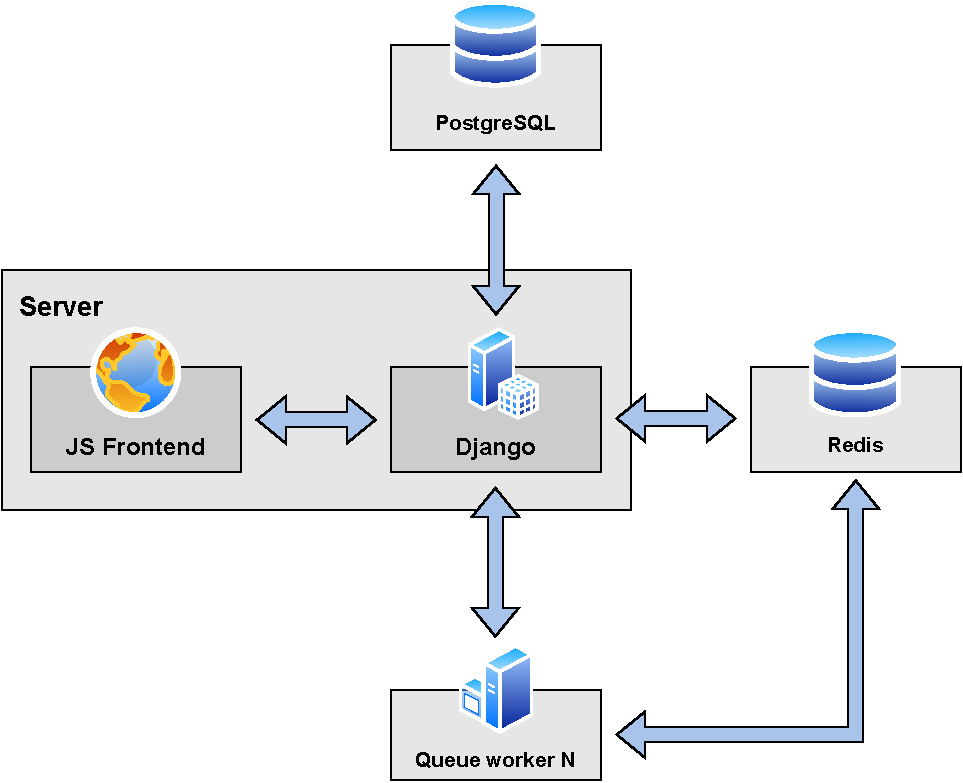
\includegraphics[width=0.85\textwidth]{resources/diagrams/kelvin-architecture}
    \caption{Zjednodušená architektura systému Kelvin}{Zjednodušená architektura systému Kelvin~\cite{kelvin-architecture}}
    \label{fig:kelvin-architecture}
\end{figure}

\endinput


% =============================================================
\section{Nasazení a provoz systému}
\label{sec:kelvin-deployment}

\input{chapters/2-kelvin/2-3-kelvin-deployment/2-3-1-kelvin-deployment-docker}

% =============================================================
\section{Vývojová omezení a proces}
\label{sec:kelvin-development}

Systém Kelvin vznikl původně jako školní projekt studenta Daniela Trnky\footnote[1]{https://github.com/trnkal}, ale v průběhu let byl postupně rozšiřován dalšími studenty a vyučujícími.
Tento způsob vývoje bez jednotné dlouhodobé architektonické vize vedl ke vzniku technického dluhu, který se v systému projevuje například ve formě dlouhých a obtížně čitelných souborů, nedostatečného nebo chybějícího typování a míchání různých programátorských přístupů.
Před přidáním nové aplikační logiky je proto často nutné provést částečný refaktoring existujícího kódu, aby byla zachována alespoň základní úroveň čitelnosti a udržovatelnosti systému.

Vývoj systému Kelvin je dále ovlivněn několika zásadními omezeními, která vyplývají jak z jeho historického vývoje, tak z organizačních podmínek jeho správy a údržby.
Tato omezení mají přímý dopad na návrh i samotnou implementaci řešení popsaného v této diplomové práci.

\subsection{Atomicita změn a code review}
\label{subsec:kelvin-development-atomicity}

Jedním z hlavních pravidel vývoje, zdokumentovaných v příručce pro rozšiřování systému\footnote[2]{\href{https://mrlvsb.github.io/kelvin/developers-guide/development\#contributing}{https://mrlvsb.github.io/kelvin/developers-guide/development\#contributing}}, je požadavek na malé a atomické pull requesty.
Každý pull request by měl obsahovat maximálně $\sim500$ změněných řádků kódu a měl by se zaměřovat pouze na jednu konkrétní změnu nebo problém.

Cílem tohoto přístupu je zjednodušení kontrolního procesu (\textit{code review}) a snížení rizika zavlečení chyb do produkčního systému.
V praxi to však znamená nutnost rozdělovat i logicky související úpravy do více menších kroků, což může celý vývojový proces prodlužovat.

\endinput

\subsection{Migrace frontendové části systému}
\label{subsec:kelvin-development-migration}

Dalším významným omezením je probíhající migrace frontendové části systému ze frameworku Svelte na framework Vue.
Při úpravách nebo přidávání nových funkcionalit by již neměly vznikat nové Svelte komponenty.
V případě rozsáhlejších změn je tak často nutné nejprve přepsat existující část aplikace do Vue a teprve následně provést požadovanou úpravu.
Tento postup výrazně zvyšuje časovou i technickou náročnost vývoje, zejména u funkcionalit zasahujících do uživatelského rozhraní.

Důvodem této migrace je zejména snaha o sjednocení technologického stacku, zlepšení dlouhodobé udržovatelnosti a snížení vstupní bariéry pro nové vývojáře systému.

\endinput

\subsection{Organizační omezení a plánování}
\label{subsec:kelvin-development-organization}

Proces schvalování změn představuje další omezení vývoje.
Neboť code review je v současné době zajišťováno omezeným počtem vyučujících, kteří se systému věnují vedle svých dalších povinností.
Z tohoto důvodu se může stát, že zpracování pull requestu (žádost o sloučení změny) trvá i několik týdnů.
Tento fakt má tím pádem dopad na tempo vývoje a vyžaduje pečlivé plánování jednotlivých kroků implementace s dostatečným časovým předstihem.

\endinput


\endinput
